\section{Introduction}
\label{introduction}

Real-time control of physical systems, like autonomous robots, raises a number of timing and control-related issues at the interface between the controller that's providing the actuation and the estimator that's providing periodic state estimates to the controller.
See Fig.~\ref{fig:codesignedCE}.
More issues arise in relation to the inaccuracies introduced by the software implementation of both controller and estimator on a given hardware platform.
Specifically, controllers are typically designed to accomplish the functional goals of the system under simplifying assumptions on the quality of the state estimate (e.g., no or fixed error), the estimation delay (e.g., no or fixed delay), or the actuation jitter (e.g., no jitter).
Note that the first effect (estimate error) is due to the estimation algorithm itself regardless of implementation, whereas the last two effects (delay and jitter) have to do with the software implementation and its characteristics on the hardware platform.
As the real-time requirements on the closed-loop system become more stringent, these assumptions are no longer valid, and a violation of the assumptions can lead to degraded performance, as we show in the example at the end of this Introduction.
It becomes important to explicitly account for (varying) estimation delays and estimation errors. 
In this paper, we take this a step further and take \emph{advantage} of the varying delay/error behavior of the estimation software to accomplish the control goals at a reduced energy cost.

Similarly, estimation algorithms are typically designed without regard to how their estimates will be used and under what operating conditions.
In particular, an estimator will often \emph{run to completion}: that is, its stopping criteria are designed to provide the best estimate, regardless of runtime or energy consumption.
%For example, the Computer Vision-based estimator we introduce in Section \ref{delayErrorCurve} uses a corner detector.
%In general, the corner detector will find the largest number of corners in a frame for best performance. 
Typical design practice determines the Worst-Case Execution Time (WCET) of the estimation task, and engineers the system to satisfy deadlines under WCET conditions.
However, the actual runtime of such estimators is heavily dependent on the actual data being processed. 
So WCET considerations, whether computed online or offline, produce a conservative design.
Moreover, classical timing analysis does not guarantee \emph{functional} correctness of the controlled system.
Indeed, even if the set of tasks of a control system is so-called schedulable, it may still fail to achieve its control objectives.
In addition, the best estimate is not always needed:
sometimes a lower quality estimate, obtained with a smaller energy cost, is sufficient to achieve the control objectives.
Finally, when obtaining better estimates requires longer runtimes of the estimation task, it may actually be detrimental to ask for the best estimate.
For example, when the computational resources are overloaded, there may be a need to spend less time computing a state estimate. 
In this paper, we provide a rigorous framework where real-time adaptation of the estimation task execution time and estimate quality allows the system to better achieve its functional goals while reducing energy consumption.
\begin{figure}[t]
	\centering
	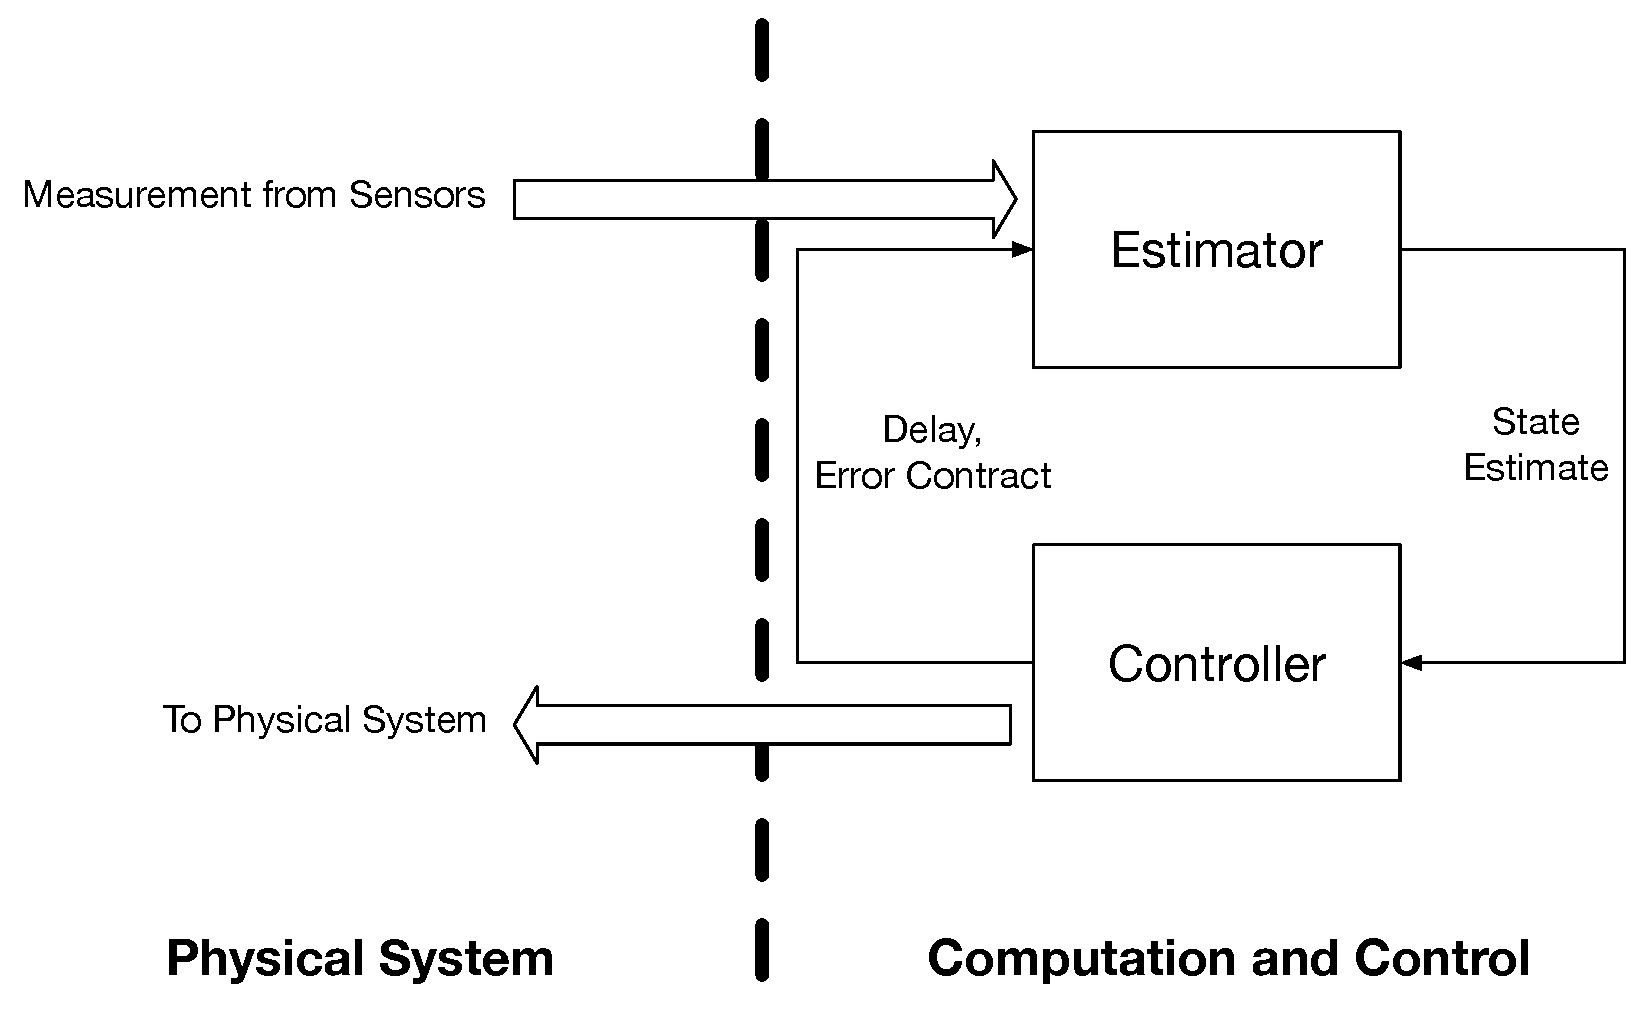
\includegraphics[width=0.9\columnwidth]{figures/omnigraffle_figures/high_level_figure.pdf}
	\caption{Contract-based co-designed controller and estimator.}
	\label{fig:codesignedCE}
\end{figure}

\subsection{Motivating Example}
\label{motivatingExample}

As a motivating example, we consider the problem of autonomous flight of a hexarotor along a pre-defined pattern.
A hexarotor is a flying robot with six rotating blades.[???]
It carries a downward facing camera that sees salient features of the environment. 
See Fig.~\ref{fig:hexarotor}.
\begin{figure}[t]
	\centering
	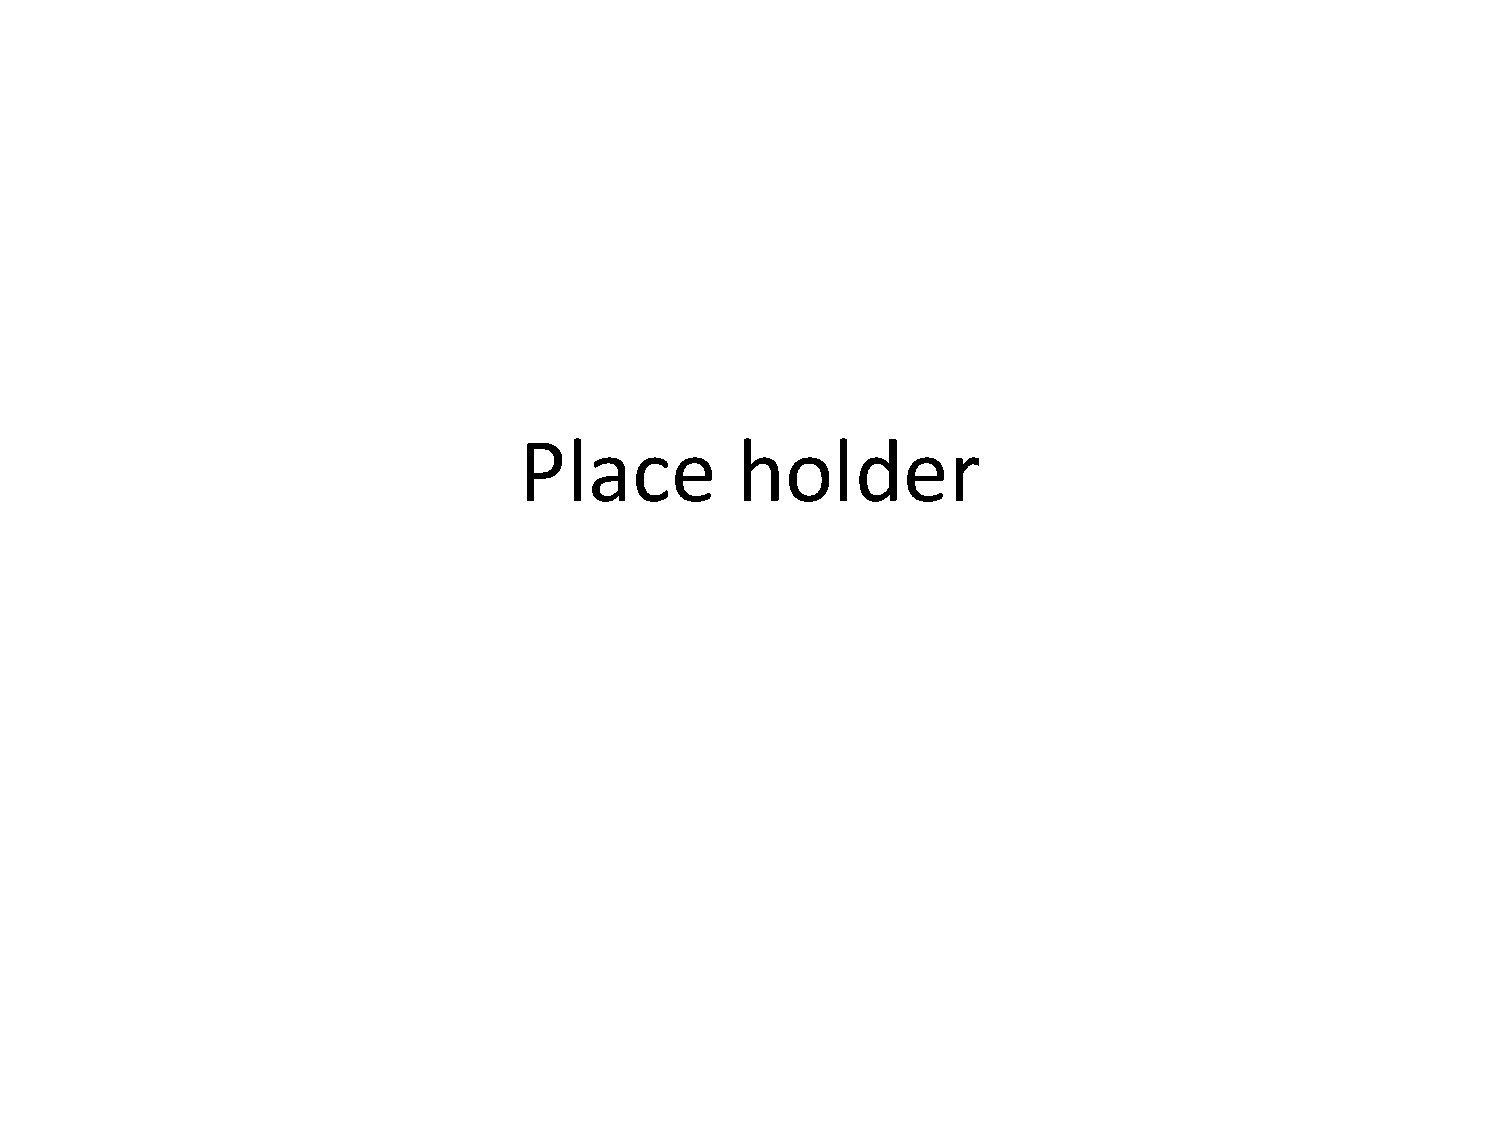
\includegraphics[width=0.7\linewidth]{figures/placeHolder}
	\caption{Hexarotor flying over synthetic features}
	\label{fig:hexarotor}
\end{figure}
These are detected by an on-board corner detector, and tracked across frames.
This allows the robot to estimate its own position in the world.
After each frame is acquired, the corner detector requires some computation time before producing its results, which are used in self-localization.
Thus the control command which uses this estimate is delayed by the time necessary to run the estimation task to completion.
This is illustrated in Fig.~\ref{fig:senseActuateDelay}.
\begin{figure}[t]
	\centering
	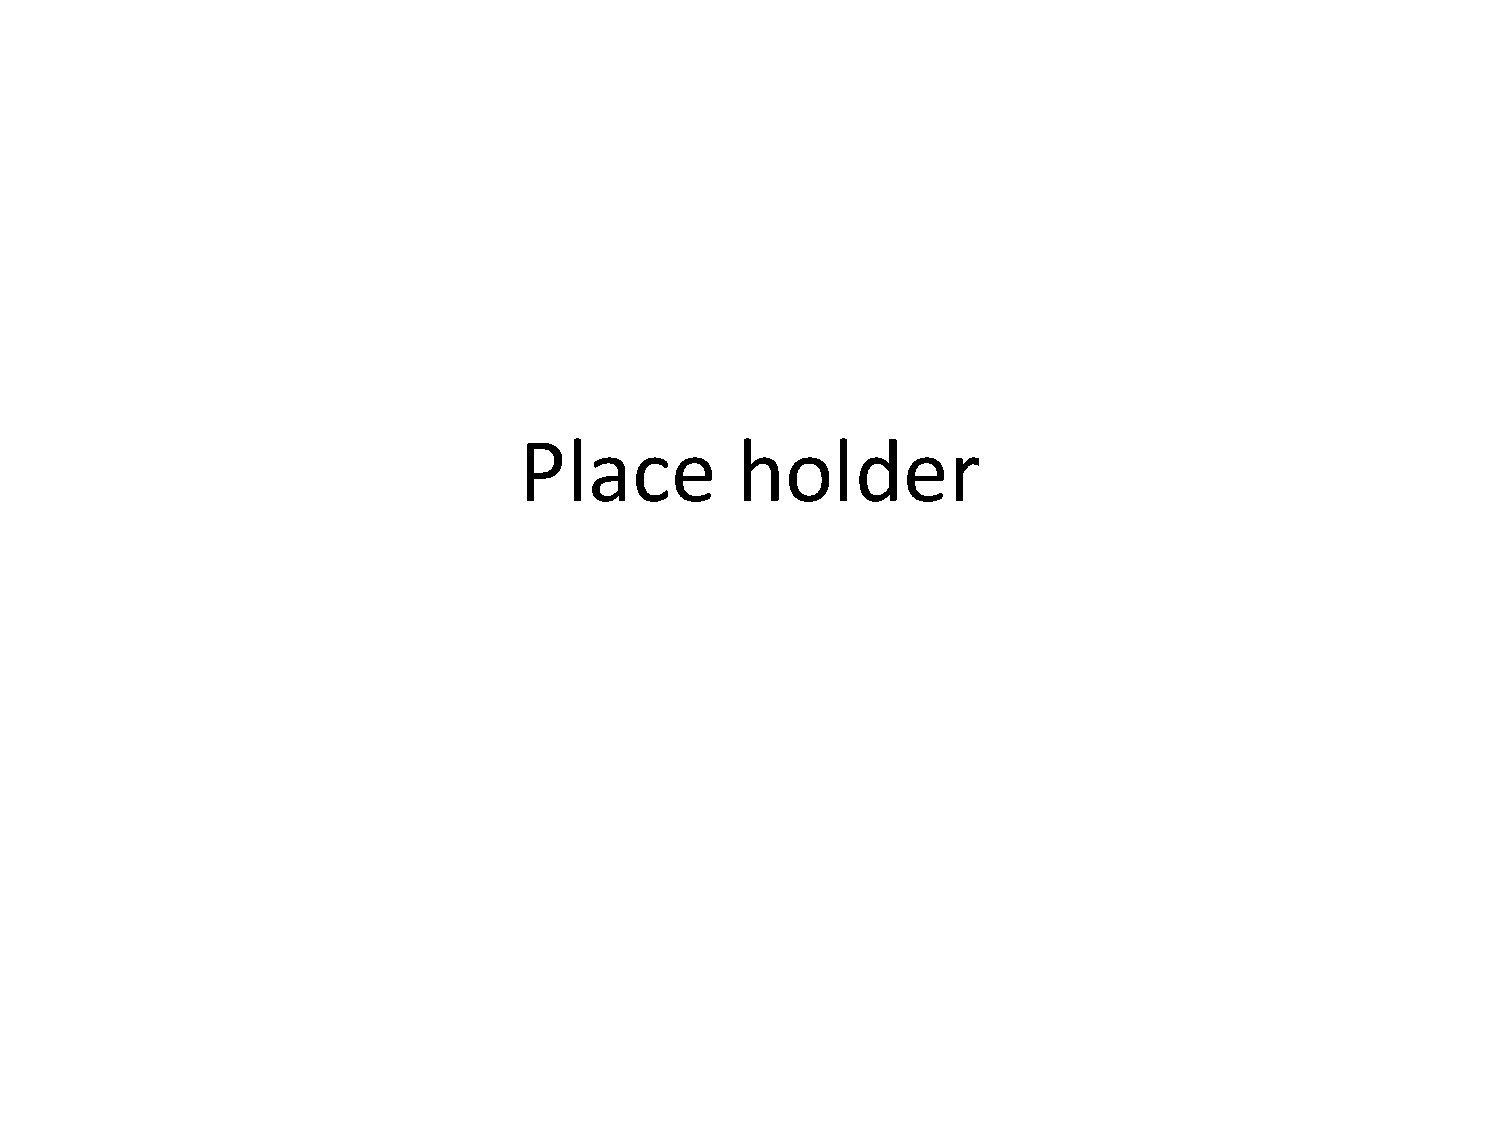
\includegraphics[width=0.7\linewidth]{figures/placeHolder}
	\caption{Sense-Estimate-Actuate cycle. The estimation task always runs to completion.}
	\label{fig:senseActuateDelay}
\end{figure}
The robot has a high-level controller which determines the desired pitch and roll angles, and desired rotor thrust. 
In this implementation, we use a Model Predictive Controller (MPC) [???].
As the robot is commanded to fly the pattern faster and faster, the estimator delay affects the control performance more.
\todo[inline]{Pending experiemental confirmation about the effect of speed of flight on control performance }
The control performance, as measured by a function that factors in the error in following the flight path and the cost of control, is shown in Fig.~\ref{fig:degradingPerformance}.
(The details of this cost function are given in Section \ref{formulation}).
\begin{figure}[t]
	\centering
	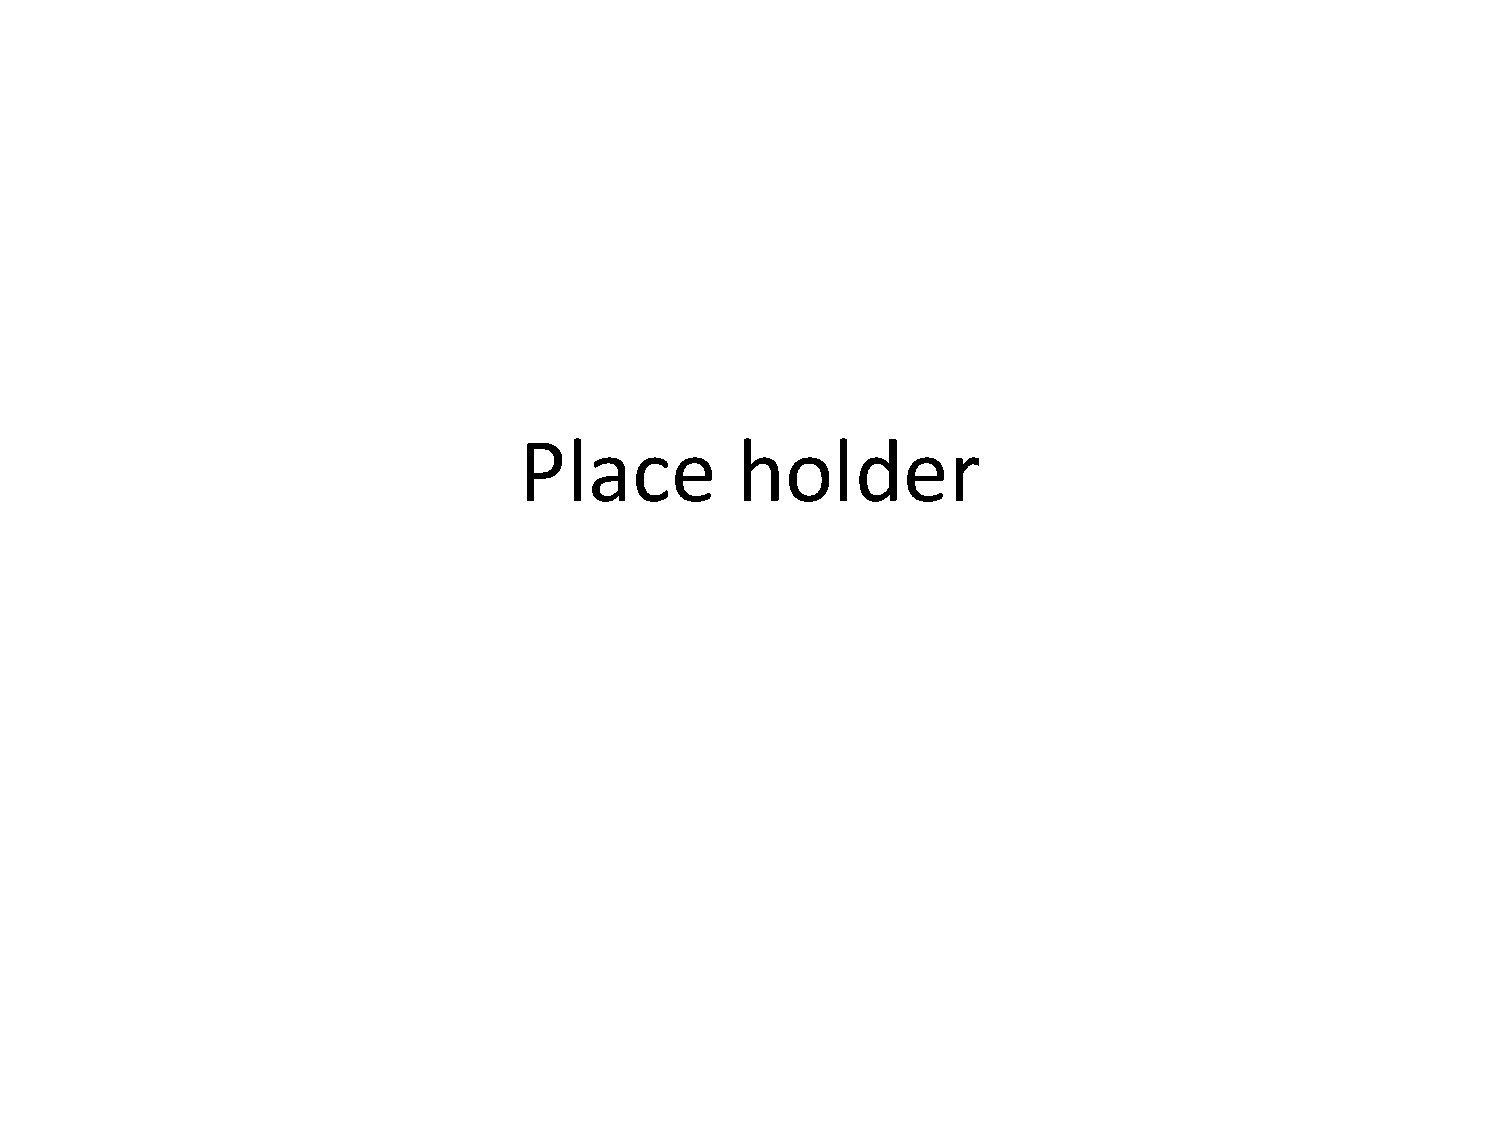
\includegraphics[width=0.7\linewidth]{figures/placeHolder}
	\caption{Degrading performance as the control objectives become more stringent.}
	\label{fig:degradingPerformance}
\end{figure}
Running an estimation task with a fixed smaller delay but larger estimation error does not necessarily solve the problem of degraded performance, as shown in Fig.~\ref{fig:degradingPerformanceSmallDelta}.
\begin{figure}[t]
	\centering
	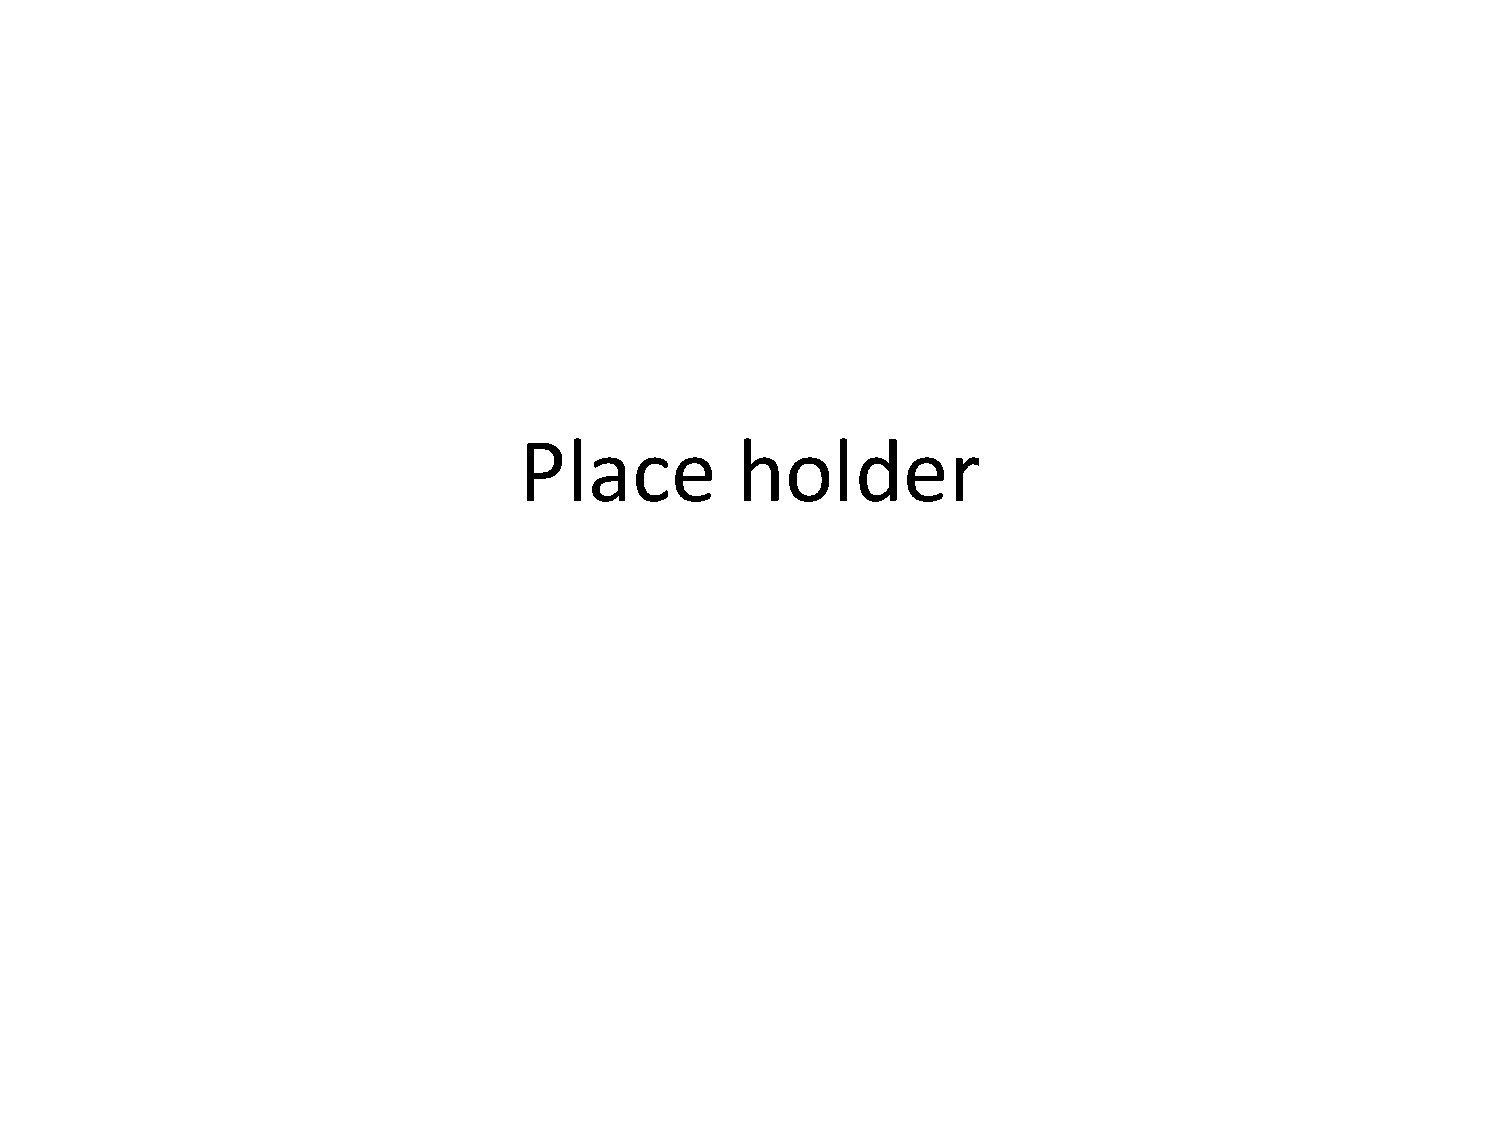
\includegraphics[width=0.7\linewidth]{figures/placeHolder}
	\caption{Degrading performance at a smaller fixed delay.}
	\label{fig:degradingPerformanceSmallDelta}
\end{figure}

Therefore, there is a need to rigorously quantify the trade-off between computation time and estimation error, then exploit that trade-off intelligently to achieve the best control performance under the problem constraints.
Rather than always run the estimation task to completion, it is useful to have several estimation tasks with varying utilities (i.e., varying delay/error trade-offs).
These can then be used at runtime to satisfy the control objectives.


In this work, we develop the above remarks into a co-design framework for a real-time control system, where the controller and estimator communicate via \emph{contracts}.
A contract is a guarantee requested by the controller, and fulfilled by the estimator, that the latter can provide an estimate with a certain maximum error $\sAccu$, and within a certain deadline $\sDelay$.
Both the accuracy and the delay are part of the contract.
Using these contracts, we show how the controller can throttle the execution time of the estimation task (i.e., estimation delay) to preserve good performance and to reduce energy consumption.
%This allows the controller to:
%1) trade-off accuracy for energy in real-time, while still being cognizant of control performance.
%2) choose the best operating mode in terms of balancing the detrimental effects of delay and accuracy on the performance.
Contract algorithms are one class of \emph{anytime} algorithms.%: algorithms that have a range of runtimes, and each runtime is associated with some quality of the algorithm's output.
Another class of anytime algorithms is called \emph{interruptible}: these are algorithms that can be interrupted at any time during their execution, and they return a usable output.[?? zilberstein]
The difference between contract and interruptible algorithms is that when the latter are interrupted, the accuracy of the output is not known beforehand to the interruptor.
Contract algorithms, on the other hand, offer a \emph{finite} number of (accuracy, delay) operating points, which constitute the `contracts'. 
When the \emph{requestor} (e.g., the controller) requests a contract, it therefore knows the accuracy with which the answer is returned.
This is important for controllers, which need to know a bound on the estimate error in order to \emph{guarantee} stability of the system and achieve functional goals.

Approximate computing approaches \cite{loop-perf,rely,npu} seek time or energy
savings by performing a computation approximately instead of precisely. While
anytime algorithms and approximate computing share a high-level goal,
approximate computing approaches are run-to-completion and also lack a feedback
mechanism to permit computation and resources to be balanced dynamically.

Recent work \cite{FrehseHQW14_Formal} uses Typical Worst Case Analysis of the software and Logical Execution Time semantics to provide the controller with knowledge of the timing characteristics of the implementation.
Our work, by contrast, profiles the estimation software directly to obtain timing and accuracy information. 
Whereas \cite{FrehseHQW14_Formal} is concerned with formal verification of a given controller, we \emph{design} controllers to take advantage of delay/accuracy trade-offs in real-time.
\todo[inline]{anthony, others?}

\textbf{Summary of contributions}.
In this work, we present a contract-based framework for the co-design of controller and estimator algorithms, consisting of:
\begin{itemize}
	\item a well-defined interface between control and estimation, in the form of operating modes or \emph{contracts} on the accuracy and delay provided by the estimator (Section \ref{sec:codesign}),
	\item a controller design that can vary the accuracy and delay of the estimation to achieve control objectives at a lower energy cost, and
	\item a general procedure to compose run-to-completion estimation algorithms into a contract-based estimator,
	\item We illustrate our approach on an autonomous flying robot and demonstrate performance and energy gains using our approach over a classical controller
\end{itemize}